% Options for packages loaded elsewhere
\PassOptionsToPackage{unicode}{hyperref}
\PassOptionsToPackage{hyphens}{url}
%
\documentclass[
  10pt,
  a4paper,
]{article}
\usepackage{amsmath,amssymb}
\usepackage{iftex}
\ifPDFTeX
  \usepackage[T1]{fontenc}
  \usepackage[utf8]{inputenc}
  \usepackage{textcomp} % provide euro and other symbols
\else % if luatex or xetex
  \usepackage{unicode-math} % this also loads fontspec
  \defaultfontfeatures{Scale=MatchLowercase}
  \defaultfontfeatures[\rmfamily]{Ligatures=TeX,Scale=1}
\fi
\usepackage{lmodern}
\ifPDFTeX\else
  % xetex/luatex font selection
  \setmainfont[]{DejaVu Sans}
  \setmonofont[]{DejaVu Sans Mono}
\fi
% Use upquote if available, for straight quotes in verbatim environments
\IfFileExists{upquote.sty}{\usepackage{upquote}}{}
\IfFileExists{microtype.sty}{% use microtype if available
  \usepackage[]{microtype}
  \UseMicrotypeSet[protrusion]{basicmath} % disable protrusion for tt fonts
}{}
\makeatletter
\@ifundefined{KOMAClassName}{% if non-KOMA class
  \IfFileExists{parskip.sty}{%
    \usepackage{parskip}
  }{% else
    \setlength{\parindent}{0pt}
    \setlength{\parskip}{6pt plus 2pt minus 1pt}}
}{% if KOMA class
  \KOMAoptions{parskip=half}}
\makeatother
\usepackage{xcolor}
\usepackage[margin=19mm]{geometry}
\usepackage{longtable,booktabs,array}
\usepackage{calc} % for calculating minipage widths
% Correct order of tables after \paragraph or \subparagraph
\usepackage{etoolbox}
\makeatletter
\patchcmd\longtable{\par}{\if@noskipsec\mbox{}\fi\par}{}{}
\makeatother
% Allow footnotes in longtable head/foot
\IfFileExists{footnotehyper.sty}{\usepackage{footnotehyper}}{\usepackage{footnote}}
\makesavenoteenv{longtable}
\usepackage{graphicx}
\makeatletter
\def\maxwidth{\ifdim\Gin@nat@width>\linewidth\linewidth\else\Gin@nat@width\fi}
\def\maxheight{\ifdim\Gin@nat@height>\textheight\textheight\else\Gin@nat@height\fi}
\makeatother
% Scale images if necessary, so that they will not overflow the page
% margins by default, and it is still possible to overwrite the defaults
% using explicit options in \includegraphics[width, height, ...]{}
\setkeys{Gin}{width=\maxwidth,height=\maxheight,keepaspectratio}
% Set default figure placement to htbp
\makeatletter
\def\fps@figure{htbp}
\makeatother
\setlength{\emergencystretch}{3em} % prevent overfull lines
\providecommand{\tightlist}{%
  \setlength{\itemsep}{0pt}\setlength{\parskip}{0pt}}
\setcounter{secnumdepth}{-\maxdimen} % remove section numbering
\ifLuaTeX
\usepackage[bidi=basic]{babel}
\else
\usepackage[bidi=default]{babel}
\fi
\babelprovide[main,import]{french}
\ifPDFTeX
\else
\babelfont{rm}[]{DejaVu Sans}
\fi
% get rid of language-specific shorthands (see #6817):
\let\LanguageShortHands\languageshorthands
\def\languageshorthands#1{}
\usepackage{etoolbox}
\usepackage{microtype}
\usepackage{float}
\floatplacement{figure}{H}
\sloppy
\setlength{\emergencystretch}{5em}
\AtBeginEnvironment{longtable}{\small}
\ifLuaTeX
  \usepackage{selnolig}  % disable illegal ligatures
\fi
\IfFileExists{bookmark.sty}{\usepackage{bookmark}}{\usepackage{hyperref}}
\IfFileExists{xurl.sty}{\usepackage{xurl}}{} % add URL line breaks if available
\urlstyle{same}
\hypersetup{
  pdftitle={Le pont arithmétique et la dette de couplage},
  pdfauthor={Vincent P. P. NOËL - dossier de recherche, rédaction assistée},
  pdflang={fr-FR},
  hidelinks,
  pdfcreator={LaTeX via pandoc}}

\title{Le pont arithmétique et la dette de couplage}
\usepackage{etoolbox}
\makeatletter
\providecommand{\subtitle}[1]{% add subtitle to \maketitle
  \apptocmd{\@title}{\par {\large #1 \par}}{}{}
}
\makeatother
\subtitle{Programme Riemann - V6.45 - Document 70}
\author{Vincent P. P. NOËL - dossier de recherche, rédaction assistée}
\date{12 octobre 2026}

\begin{document}
\maketitle

{
\setcounter{tocdepth}{2}
\tableofcontents
}
\hypertarget{le-ruxe9sultat-de-cette-uxe9tape}{%
\section{1. Le résultat de cette
étape}\label{le-ruxe9sultat-de-cette-uxe9tape}}

L'étape relie l'admissibilité des tests à la partie première de la forme
complète. Les deux moments exponentiels annulent un noyau polaire de
rang deux. Le terme continu des premiers devient alors une énergie de
graine de signe connu. La fluctuation de Chebyshev reste dans une forme
signée exacte. Cela précise ce qui doit apporter le signe global.

Deux obstructions sont également démontrées : le modèle continu corrigé
seul n'est pas positif sur tous les supports ; un nombre fini de moments
ne diminue pas la norme L² de l'opérateur premier. Elles ferment deux
raccourcis possibles.

Le nouveau contrat de Schur contrôle la dette par un Gram de
\textbf{résidus de sources}. Il fonctionne avec une tête non orthogonale
et évite un solveur Riesz exact, si les erreurs des sources sont
encadrées. Il demeure un certificat suffisant, avec une obligation de
régularité distincte pour sa convergence.

L'expérience exécute 144 entrées triangulaires premières/résiduelles
avec intervalles binaires, quatre budgets de queue améliorés et six
témoins de modèle continu. Le signe archimédien total des compressions
reste celui du diagnostic V644, sans être promu en certificat par ces
nouveaux encadrements.

La destination demeure le signe du Schur pour tous les supports. Aucune
preuve de RH ni priorité bibliographique des identités reconstruites
n'est revendiquée.

\hypertarget{objets-unituxe9s-et-domaines}{%
\section{2. Objets, unités et
domaines}\label{objets-unituxe9s-et-domaines}}

Pour \(S>0\), \(D=2S\), \(I=(-S,S)\), \[
P=\partial_x^2-\tfrac14,\quad f=P\psi,\quad
\ell_\pm(f)=\int_I f(x)e^{\pm x/2}dx=0.
\] Sur le domaine H¹ admissible E\_S et sa complétion logarithmique X\_S
de V644, \[
Q_W=\mathcal E-C_0\|f\|_2^2-Q_{\rm pr},\quad
\mathcal E(f)=\int_0^\infty w(t)\|U_tf-f\|_2^2dt,
\quad w(t)=\frac{e^{-t/2}}{1-e^{-2t}},
\] \[
C_0=\log(8\pi)+\gamma_E+\pi/2.
\] \[
Q_{\rm pr}(f)=2\sum_{p^m\le e^D}\frac{\log p}{p^{m/2}}\Re h_f(m\log p),
\] \[
h_f(t)=\int f(y)\overline{f(y-t)}dy.
\] Le produit scalaire est antilinéaire en première variable.
R=masse+énergie de déplacement est la métrique externe, indépendante des
premiers et du signe recherché.

La fonction de Chebyshev est nommée \(\Psi\), la graine \(\psi\) : \[
\Psi(x)=\sum_{p^m\le x}\log p,\qquad
\Delta_\Psi(t)=\Psi(e^t)-e^t+1,\qquad \Delta_\Psi(0)=0.
\] La distinction évite de confondre trois ψ : graine, fonction de
Chebyshev, et digamma utilisée dans des contrôles de Fourier.

x,t,S sont logarithmiques sans dimension ; Ψ et ΔΨ portent unité 1. Les
graines, tests et sources portent \(A_{\rm amp}\), toutes les formes et
Grams portent \(E=A_{\rm amp}^2\). Les β, μ et coefficients de dette
sont sans dimension. La lettre E d'une unité est distincte de l'énergie
archimédienne \(\mathcal E\).

\hypertarget{c1---ladmissibilituxe9-donne-le-signe-du-terme-continu}{%
\section{3. C1 - L'admissibilité donne le signe du terme
continu}\label{c1---ladmissibilituxe9-donne-le-signe-du-terme-continu}}

\textbf{Énoncé.} Sur le domaine admissible, \[
Q_{\rm cont}(f):=2\int_0^D e^{t/2}\Re h_f(t)dt=-P_0(f),
\quad P_0(f)=\int_{\mathbb R}\frac{|\widehat f(\tau)|^2}{\tau^2+1/4}d\tau\ge0.
\] Si f=Pψ, alors \[
\boxed{P_0(f)=\|\psi'\|_2^2+\tfrac14\|\psi\|_2^2.}
\] \textbf{Preuve.} L'identité de noyaux \[
e^{|x-y|/2}=2\cosh((x-y)/2)-e^{-|x-y|/2}
\] sépare une forme de rang deux. La contribution de cosh est
\(\Re(\overline{\ell_+(f)}\ell_-(f))\), donc zéro. La contribution
restante est l'opposé de la forme du noyau \(e^{-|x|/2}\), dont le
multiplicateur Fourier est \((\tau^2+1/4)^{-1}\). Plancherel donne la
formule. Comme \(\widehat f=-(\tau^2+1/4)\widehat\psi\), sa valeur est
l'énergie annoncée.

Autre vérification : \(P e^{|x|/2}=\delta_0\), le saut de la dérivée
valant 1. Les moments annulent les queues de \(e^{|\cdot|/2}*f\), qui
est donc ψ par l'unicité de l'inverse compact de P. L'intégration par
parties donne \(\langle P\psi,\psi\rangle=-\|\psi'\|^2-\|\psi\|^2/4\). □

La preuve en noyau vaut pour les tests L² de support fixé avec deux
moments nuls. Pour f∈X\_S, l'inverse compact est H₀² ; l'identité
s'étend sans supposer H¹. Le coup double est exact : les mêmes
contraintes ferment le domaine et annulent la partie polaire qui
masquait le signe du modèle continu.

\hypertarget{c2---la-fluctuation-premiuxe8re-garde-la-dette-arithmuxe9tique}{%
\section{4. C2 - La fluctuation première garde la dette
arithmétique}\label{c2---la-fluctuation-premiuxe8re-garde-la-dette-arithmuxe9tique}}

Poser \(H_f=\Re h_f\), \(F_f(t)=e^{-t/2}H_f(t)\). La mesure première est
\(d\Psi(e^t)\), avec masses log p en t=m log p. L'identité de mesures
\(d\Psi(e^t)=e^tdt+d\Delta_\Psi(t)\) donne \[
Q_{\rm pr}(f)=-P_0(f)+2\int_{[0,D]}F_f(t)\,d\Delta_\Psi(t).
\] Pour f∈H¹, H\_f est C¹ ; F\_f(D)=0 et ΔΨ(0)=0. L'intégration par
parties donne \[
\boxed{Q_W(f)=B_0(f)+\mathfrak F_\Psi(f),}
\] \[
B_0(f)=\mathcal E(f)-C_0\|f\|_2^2+P_0(f),\qquad
\mathfrak F_\Psi(f)=2\int_0^D\Delta_\Psi(t)e^{-t/2}
\bigl(H_f'(t)-H_f(t)/2\bigr)dt.
\] Il n'y a aucun terme de bord manquant. Pour X\_S, utiliser la forme
de Stieltjes avant dérivation : corrélation continue et mesure de
variation finie suffisent. La version avec H′ demande la garde H¹. □

Cette traduction conserve exactement la forme et son signe : elle ne
remplace pas les premiers par une moyenne. Elle isole leur fluctuation
signée après l'annulation du terme polaire. La formule bilinéaire suit
par polarisation ; pour une base réelle, les matrices symétrisées
donnent toute combinaison complexe.

\hypertarget{c3---deux-raccourcis-fermuxe9s}{%
\section{5. C3 - Deux raccourcis
fermés}\label{c3---deux-raccourcis-fermuxe9s}}

\hypertarget{le-moduxe8le-continu-seul-nest-pas-positif-globalement}{%
\subsection{Le modèle continu seul n'est pas positif
globalement}\label{le-moduxe8le-continu-seul-nest-pas-positif-globalement}}

Soit une graine non nulle lisse intérieure et
\(\psi_S(x)=S^{-1/2}\psi(x/S)\), \(f_S=P\psi_S\). Ces tests sont
admissibles. L'inégalité \(\mathcal E(f)\le C_2\|f'\|_2^2\),
\(C_2=\int_0^\infty t^2w(t)dt<\infty\), donne \(\mathcal E(f_S)\to0\).
Ainsi \[
\frac{B_0(f_S)}{\|f_S\|_2^2}\longrightarrow4-C_0<0.
\] Une borne élémentaire suffit pour le signe : π\textgreater3, γ\_E≥0
et \(\log(8\pi)>\log16=4\log2\ge8/3\), donc \(C_0>25/6>4\). La
fluctuation doit apporter une compensation basse fréquence ; elle ne
peut être déclarée uniformément négligeable.

\textbf{Témoins rationnels.} Pour la graine polynomiale de V644,
\(\psi=w_S=(1-x^2/S^2)^4\), f=Pψ, les masses et P₀ sont rationnels. Le
développement positif du noyau donne \[
C_2=\sum_{n\ge0}\frac2{(2n+1/2)^3}
\le16+\tfrac14\sum_{n\ge1}n^{-3}\le\frac{131}8.
\] Donc \[
B_0(f)\le\frac{131}8\|f'\|_2^2-\frac{25}6\|f\|_2^2+P_0(f).
\] Le tableau d'exécution fournit des bornes supérieures rationnelles
négatives dès certains supports prédéclarés. Elles réfutent la
positivité du modèle B₀ ; elles ne sont pas des témoins négatifs de
Q\_W.

\textbf{Renforcement uniforme démontré après l'exécution.} Poser
\(A_j=\int_{-1}^1|D^j(1-u^2)^4|^2du\). L'intégration polynomiale exacte
donne \[
(A_0,A_1,A_2,A_3)=
\left(\frac{65536}{109395},\frac{131072}{45045},
\frac{196608}{5005},\frac{65536}{77}\right).
\] Si U(S) désigne le majorant de B₀ affiché ci-dessus, les changements
d'échelle et les intégrations par parties donnent \[
\frac{U(S)}S=-\frac{A_0}{96}-\frac{23A_1}{384S^2}
+\frac{193A_2}{48S^4}+\frac{131A_3}{8S^6}.
\] Pour S≥16, supprimer le terme négatif en S⁻² et majorer les deux
termes positifs par leur valeur en 16 donne \[
\boxed{\frac{B_0(Pw_S)}S\le\frac{U(S)}S
\le-\frac{14112607}{4704860160}<0\quad(S\ge16).}
\] Il s'agit d'une obstruction sur tout un régime de supports, pas d'une
extrapolation des six calculs. La preuve concerne toujours B₀ seul. □

\hypertarget{les-moments-ne-rendent-pas-les-premiuxe8res-translations-petites-en-luxb2}{%
\subsection{Les moments ne rendent pas les premières translations
petites en
L²}\label{les-moments-ne-rendent-pas-les-premiuxe8res-translations-petites-en-luxb2}}

Sur L²(I), soit \(K_{\rm pr}=\sum_a w_a\Pi_I(U_a+U_{-a})\Pi_I\),
w\_a\textgreater0. Pour le noyau M d'un nombre fini de fonctionnelles L²
continues, \[
\sup_{f\in M,\ \|f\|_2=1}\langle f,K_{\rm pr}f\rangle=\|K_{\rm pr}\|.
\] \textbf{Preuve.} Le noyau de translations est positif au sens de
préservation des fonctions non négatives ;
\(|\langle f,Kf\rangle|\le\langle|f|,K|f|\rangle\). On peut donc
approcher sa norme par une enveloppe lisse non négative φ. Une
récurrence simultanée sur le tore fournit τ\_j→∞ avec
\(e^{i\tau_j a}\to1\) pour le nombre fini de décalages a. Le Rayleigh de
\(e^{i\tau_jx}\phi\) revient vers celui de φ. Ses moments tendent vers
zéro par Riemann--Lebesgue. Des fonctions duales fixes les corrigent
exactement avec une erreur L² tendant vers zéro. La continuité L² de K
conserve la limite. Si les fonctionnelles sont dépendantes, garder une
base de leur span pour cette correction. □

Le mot positif ci-dessus signifie préservation de fonctions positives,
pas forme quadratique positive. Le mécanisme démontre pourquoi la
métrique R ou une garde de bande reste nécessaire : elle fait payer les
hautes fréquences.

\hypertarget{c4---des-budgets-issus-du-support-avec-intervalle-de-queue}{%
\section{6. C4 - Des budgets issus du support, avec intervalle de
queue}\label{c4---des-budgets-issus-du-support-avec-intervalle-de-queue}}

Pour un décalage a\textgreater0, D longueur de I, \[
\|\Pi_I(U_a+U_{-a})\Pi_I\|
=2\cos\frac\pi{\lceil D/a\rceil+1}.
\] \textbf{Preuve.} Décomposer x=r+ka selon les fibres modulo a. Les
translations deviennent l'adjacence d'une chaîne. La plus grande
longueur de chaîne sur un ensemble de fibres de mesure positive est
\(\lceil D/a\rceil\). La norme d'une chaîne de n sommets vaut
\(2\cos(\pi/(n+1))\). À a=D, elle est zéro. □

Cela améliore la somme brute de V644. Une autre borne est le test de
Schur par sommes de lignes : \[
\|K_{\rm pr}\|\le\operatorname*{ess\,sup}_{0<x<D}
\{A(x)+A(D-x)\},\quad A(u)=\sum_{a\le u}w_a.
\] Les candidats de ce supremum se calculent avec des produits entiers :
\(\log n+\log m\le D\iff nm\le e^D\). Pour les supports rationnels du
protocole, un plafond encadré décide toutes les comparaisons. Ces bornes
concernent l'opérateur \textbf{comprimé sur I} ; c'est bien celui qui
intervient entre deux tests de X\_S. Elles ne sont pas annoncées pour
les translations sur toute la droite.

La constante retenue L majore \((C_0+1)I+K_{\rm pr}\) sur L²(I). Pour
accélérer le contrat de queue, écrire \[
a(T)=\sum_{n\ge0}\frac{2T^2}{b_n(b_n^2+T^2)},\qquad b_n=2n+\tfrac12.
\] Les termes décroissent en n.~Pour K≥0, si A\_K est la somme
n\textless K, \[
A_K+\tfrac12\log(1+T^2/b_K^2)
\le a(T)\le A_K+\tfrac12\log(1+T^2/b_K^2)
+\frac{2T^2}{b_K(b_K^2+T^2)}.
\] Ces encadrements suivent de la comparaison série/intégrale, sans
coupure archimédienne arbitraire. La boucle cherche T=2\^{}J avec
r\_lower=1+a\_lower\textgreater2L. Avec q=ceil(6ST), V644 donne ε≤1/12,
donc \[
\beta\le\frac{12}{11r_{\rm lower}},\qquad
\mu\ge1-L\beta>0\quad\text{sur }Y_{q-1}.
\] Les γ\_E sont encadrés par
\(H_n-\log n-1/n\le\gamma_E\le H_n-\log n\), n=1024. Les quotients et
marges sont stockés en fractions exactes à partir des bornes binaires.
La tête de dimension q n'est pas pour autant calculée.

\hypertarget{c5---la-dette-de-schur-devient-un-gram-de-ruxe9sidus}{%
\section{7. C5 - La dette de Schur devient un Gram de
résidus}\label{c5---la-dette-de-schur-devient-un-gram-de-ruxe9sidus}}

Supposer les deux contrats de queue \[
Q_W(y)\ge\mu R(y),\qquad\|y\|_2^2\le\beta R(y),\quad y\in Y_N,\quad\mu>0.
\] Choisir un complément de Y\_N avec q=N+1 représentants v\_i, et les
améliorer par \(h_i=v_i+y_i\), y\_i∈Y\_N. Pour ce calcul, exiger
h\_i∈H¹. Leur source forte, restreinte à I, est \[
k_i=\int_0^\infty w(t)(2h_i-U_th_i-U_{-t}h_i)dt
-C_0h_i-\sum_a w_a(U_a+U_{-a})h_i.
\] Elle est L² : près de zéro, la norme de la différence est
≤2t\textbar\textbar h\_i′\textbar\textbar, intégrable contre w ; la
queue est intégrable. Pour des fonctions véritables
\(p_i\in\operatorname{span}\{1,x,\ldots,x^N,e^{x/2},e^{-x/2}\}\) sur I,
poser ρ\_i=k\_i−p\_i. Elles donnent
\(Q_W(h_i,y)=\langle\rho_i,y\rangle_2\), puisque p\_i annihile Y\_N.
Avec \(H_{ij}=Q_W(h_i,h_j)\), \(C_{ij}=\langle\rho_i,\rho_j\rangle_2\),
\[
\boxed{H-\frac\beta\mu C\ \preceq\ G_{\rm eff,S}\ \preceq H.}
\] \textbf{Preuve.} Pour h=Σc\_ih\_i et y∈Y\_N,
\(|Q_W(h,y)|\le\sqrt\beta\|\sum c_i\rho_i\|_2\|y\|_R\). Compléter le
carré avec \(Q_W(y)\ge\mu\|y\|_R^2\) borne la dette par
\(\beta c^*Cc/\mu\). Le choix y=0 donne le majorant H. Changer h\_i par
un élément de sa classe modulo Y\_N conserve le Schur exact. Aucune
orthogonalité R du complément n'est requise. □

Ainsi \[
H-(\beta/\mu)C\succeq0\quad\Longrightarrow\quad Q_W\ge0\text{ sur tout }X_S.
\] Le coup double consiste à améliorer les représentants de tête et à
mesurer leurs couplages par des résidus explicites. Le solveur Riesz
exact et l'inverse de queue ne sont plus requis pour ce certificat
suffisant.

\hypertarget{version-robuste-aux-erreurs}{%
\subsection{Version robuste aux
erreurs}\label{version-robuste-aux-erreurs}}

Si \textbar\textbar H−Htilde\textbar\textbar≤δ\_H,
\textbar\textbar Ctilde−Gram(ρtilde)\textbar\textbar≤δ\_C et
\textbar\textbar ρ\_i−ρtilde\_i\textbar\textbar₂≤ε\_i, alors, pour
θ\textgreater0, \[
C_{\rm up}=(1+\theta)(\widetilde C+\delta_C I)
+(1+\theta^{-1})\Bigl(\sum_i\varepsilon_i^2\Bigr)I.
\] La condition \[
\widetilde H-\delta_HI-(\beta/\mu)C_{\rm up}\succeq0
\] suffit. Elle suit de Cauchy--Schwarz et Young ; les erreurs de Gram
sont conservées. Pour sources exactes, employer simplement C+δ\_CI. Une
procédure rationnelle vérifie cette algèbre matricielle ; son résultat
exige encore les contrats analytiques, une tête complète et les normes
d'erreur validées.

\hypertarget{garde-de-convergence}{%
\subsection{Garde de convergence}\label{garde-de-convergence}}

La densité dans R n'assure pas que les résidus de sources convergent en
L². Le vrai résidu dual R* peut converger sans que ce majorant L² tende
vers zéro. Ce certificat est suffisant ; sa terminaison n'est pas
démontrée. Une régularité du minimiseur ou une approximation en norme de
graphe de la source est une obligation distincte. Une erreur sur grille
ne vaut pas norme L² encadrée.

\hypertarget{exuxe9cution-encadrements-et-compensations}{%
\section{8. Exécution, encadrements et
compensations}\label{exuxe9cution-encadrements-et-compensations}}

Le protocole a précédé les évaluations V645. Les matrices V644 et leur
signe observé étaient déjà connus ; leur nouvelle décomposition est
explicitement une réanalyse. Les directions proposées ensuite par le
minimum de B₀ sont étiquetées comme analyse après décomposition, avec
coefficients rationnels.

\begin{longtable}[]{@{}
  >{\raggedright\arraybackslash}p{(\columnwidth - 6\tabcolsep) * \real{0.2500}}
  >{\raggedright\arraybackslash}p{(\columnwidth - 6\tabcolsep) * \real{0.2500}}
  >{\raggedright\arraybackslash}p{(\columnwidth - 6\tabcolsep) * \real{0.2500}}
  >{\raggedright\arraybackslash}p{(\columnwidth - 6\tabcolsep) * \real{0.2500}}@{}}
\toprule\noalign{}
\begin{minipage}[b]{\linewidth}\raggedright
S
\end{minipage} & \begin{minipage}[b]{\linewidth}\raggedright
L brut encadré
\end{minipage} & \begin{minipage}[b]{\linewidth}\raggedright
L retenu, majorant
\end{minipage} & \begin{minipage}[b]{\linewidth}\raggedright
chiffres de q : V644 → V645
\end{minipage} \\
\midrule\noalign{}
\endhead
\bottomrule\noalign{}
\endlastfoot
1/2 & {[}7.3519, 7.3530{]} & 6.8629 & 25 → 5 \\
1 & {[}12.2241, 12.2252{]} & 9.2990 & 45 → 8 \\
2 & {[}30.7549, 30.7560{]} & 18.5644 & 136 → 16 \\
3 & {[}81.5621, 81.5632{]} & 43.9680 & 493 → 38 \\
\end{longtable}

L'encadrement de γ rend les constantes de norme légèrement épaisses ;
les extrémités binaires, et non les décimales d'affichage, décident le
contrat. Pour S=3, la tête passe de 493 chiffres à 38 chiffres. Ce
progrès est démontré, mais sa taille demeure prohibitive pour un calcul
direct.

\begin{longtable}[]{@{}
  >{\raggedright\arraybackslash}p{(\columnwidth - 4\tabcolsep) * \real{0.3333}}
  >{\raggedright\arraybackslash}p{(\columnwidth - 4\tabcolsep) * \real{0.3333}}
  >{\raggedright\arraybackslash}p{(\columnwidth - 4\tabcolsep) * \real{0.3333}}@{}}
\toprule\noalign{}
\begin{minipage}[b]{\linewidth}\raggedright
S
\end{minipage} & \begin{minipage}[b]{\linewidth}\raggedright
borne supérieure rationnelle de B₀ / masse, affichée vers le haut
\end{minipage} & \begin{minipage}[b]{\linewidth}\raggedright
signe négatif certifié
\end{minipage} \\
\midrule\noalign{}
\endhead
\bottomrule\noalign{}
\endlastfoot
4 & 14.202134 & non tranché par cette borne \\
8 & 1.186309 & non tranché par cette borne \\
16 & -0.084171 & oui \\
32 & -0.160588 & oui \\
64 & -0.165961 & oui \\
128 & -0.166539 & oui \\
\end{longtable}

\begin{longtable}[]{@{}llll@{}}
\toprule\noalign{}
S & B₀, diagnostic & fluctuation, intervalle & Q complet, diagnostic \\
\midrule\noalign{}
\endhead
\bottomrule\noalign{}
\endlastfoot
1/2 & 0.0012854137 & {[}0.00000337, 0.00000338{]} & 0.0012887901 \\
1 & -0.01816352 & {[}0.01827853, 0.01827854{]} & 0.00011501748 \\
2 & -0.15802279 & {[}0.15814225, 0.15814226{]} & 0.00011946339 \\
3 & -0.38642924 & {[}0.38645831, 0.38645832{]} & 2.907639e-05 \\
\end{longtable}

\begin{figure}
\centering
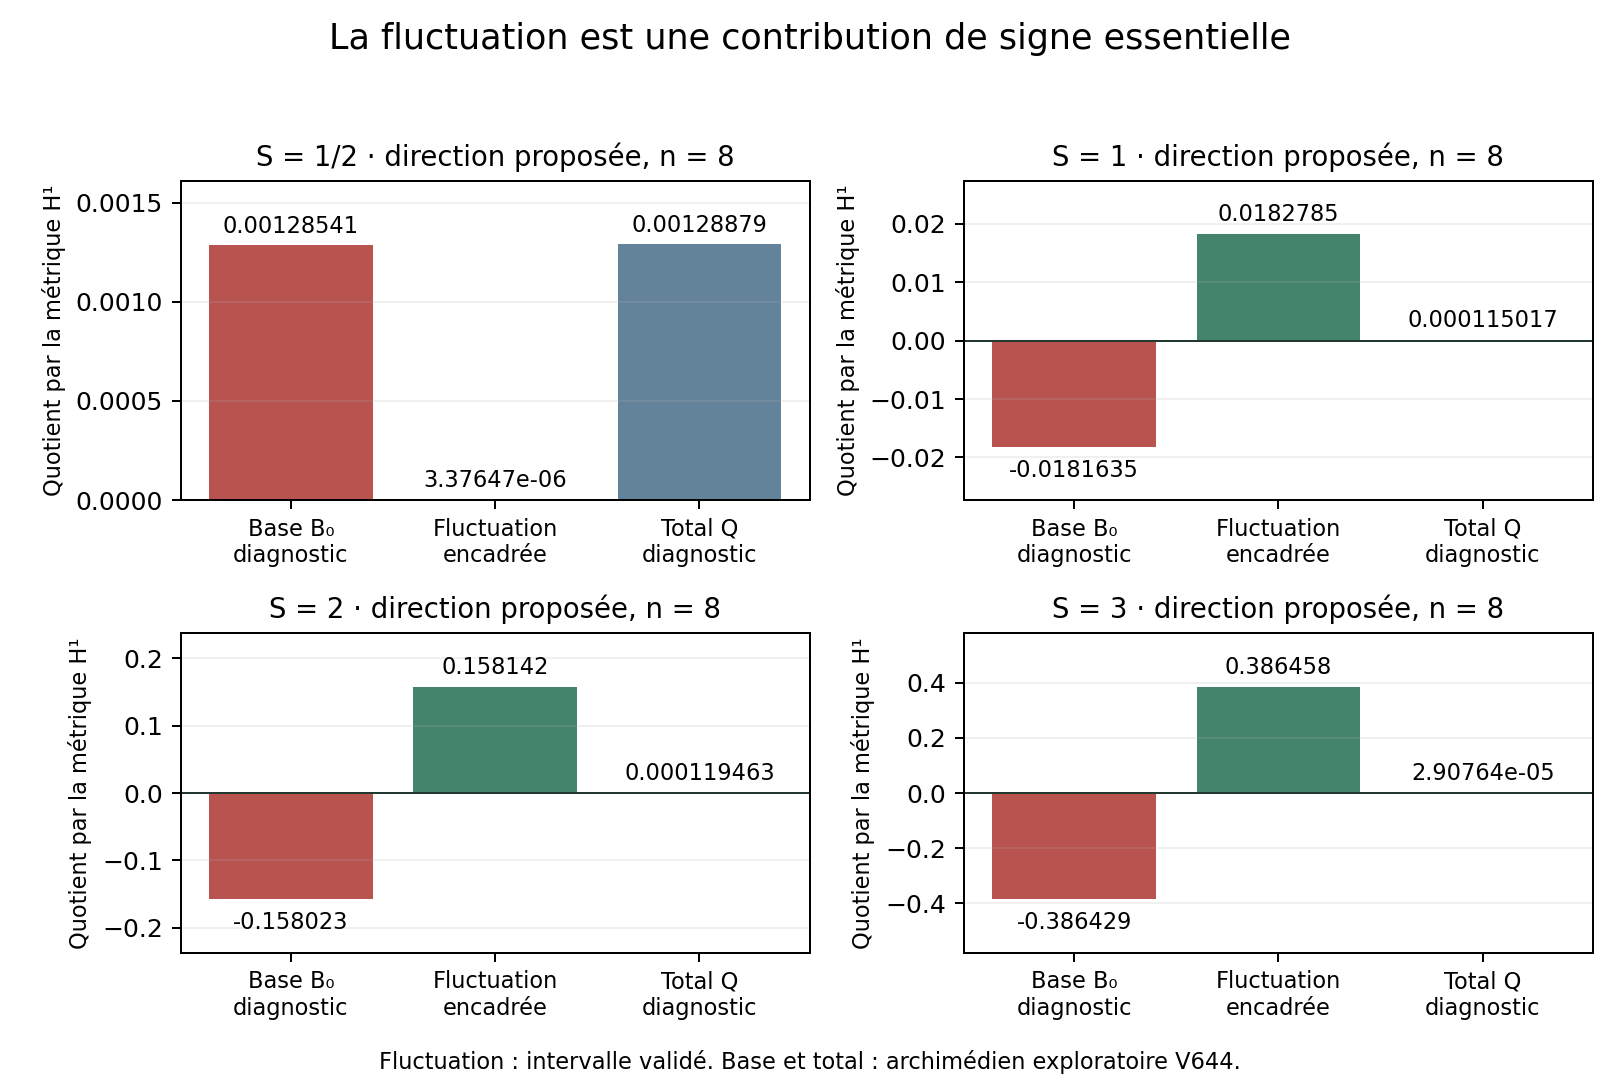
\includegraphics{70_COMPENSATION_ARITHMETIQUE.png}
\caption{Compensation dans les directions proposées.}
\end{figure}

La fluctuation dans les directions affichées a un signe encadré. La base
et la somme totale utilisent encore les valeurs archimédiennes
exploratoires de V644. Le signe de la somme n'est donc pas certifié par
cette expérience.

Les 144 coefficients triangulaires ont été calculés par deux voies :
somme première directe et primitive exponentielle de l'intégration par
parties, par intervalles à 400 bits. L'énergie de graine est
rationnelle. Les intervalles des deux voies se recouvrent, et le terme
continu contient exactement −P₀. L'algorithme sauvegarde les bornes
binaires ; les erreurs maximales et la reconstruction de Q figurent dans
le journal JSON. Les fonctions élémentaires à arrondi d'intervalles sont
celles du même environnement mpmath.iv que V636. Ce contrôle ne
constitue pas un nouveau certificat de la quadrature archimédienne.

\hypertarget{la-loi-arithmuxe9tique-qui-manque}{%
\section{9. La loi arithmétique qui
manque}\label{la-loi-arithmuxe9tique-qui-manque}}

La nouvelle identité exige que la fluctuation soit contrôlée
\textbf{avec sa phase, ses corrélations et ses couplages}. Une borne
absolue de taille peut perdre la compensation qui fait vivre le signe.
Le contrat global est désormais explicite : pour chaque S, produire une
tête complète, un contrat de queue et des résidus, avec une matrice
inférieure positive. Une loi arithmétique couvrant toute cette famille
fermerait le signe global.

Ne pas importer comme hypothèse la borne
\(\Psi(x)-x=O(x^{1/2+\varepsilon})\) pour tout ε\textgreater0 : le DLMF
§25.16 la donne déjà comme équivalente à RH. Notre identité est prouvée
sans cette borne. Le théorème des nombres premiers seul ne contrôle pas
le signe de toutes les corrélations admissibles.

La prochaine enquête a deux portes ET : encadrer les sources h\_i et
leurs résidus, et trouver une représentation de tête dont la taille et
la dette restent contrôlables. Il faut préparer des quadratures Bochner
avec erreurs L² et une approximation des annihilateurs, puis confronter
H−βC/μ au signe. Une loi couvrante reste nécessaire au-delà de tout
certificat de support particulier.

Succès local : certificat analytique et matriciel complet pour le S
choisi. Refutation : témoin négatif encadré de la forme complète, sous
toutes les gardes. Issue indéterminée : erreur ou borne manquante
identifiée. Une base B₀ négative ne remplit pas le critère de réfutation
de RH.

\hypertarget{lecture-primaire-et-portuxe9e}{%
\section{10. Lecture primaire et
portée}\label{lecture-primaire-et-portuxe9e}}

Connes et Consani {[}CC21{]}, \emph{Weil positivity and Trace formula,
the archimedean place} (2021), §3, proposition 3.5 et théorème 3.6 : le
passage aux moments par opérateur différentiel, puis identité signée
plus compact, apparaît déjà dans le traitement archimédien. Cette
lecture précise l'ancrage conceptuel de nos traductions ; elle ne
transfère pas leur positivité restreinte à tous les premiers. Texte
auteur :
\href{https://alainconnes.org/wp-content/uploads/Selecta.pdf}{alainconnes.org}.

NIST {[}NIS26{]}, DLMF §25.16(i), équations 25.16.1, 25.16.3 et 25.16.4
: définition de Ψ, théorème des nombres premiers et borne équivalente à
RH. Les constantes du nouveau calcul n'utilisent pas cette dernière
hypothèse. \href{https://dlmf.nist.gov/25.16}{Source}.

Un préprint de juillet 2026, \emph{A finite Guinand-Weil dictionary and
archimedean tail order for the truncated Weil quadratic form},
arXiv:2607.02828, a été repéré et son résumé lu {[}Gro26{]}. Son
dictionnaire est limité à une troncature et une bande ; sa preuve et ses
artefacts restent à auditer avant usage. Il n'est pas utilisé comme
prémisse de nos certificats.

Les preuves C1--C5 ont fait l'objet d'une lecture constructive et d'une
lecture critique, avec accords sur les domaines, les signes et les
obstructions. Les noms nouveaux organisent des structures classiques ;
la priorité dans la littérature n'est pas revendiquée. V644, documents
68--69, conserve ses preuves et sa grammaire. Les branches, collisions
et paramètres complexes des autres familles restent ouverts dans leur
portée propre.

\hypertarget{ruxe9fuxe9rences}{%
\subsection{Références}\label{ruxe9fuxe9rences}}

Format : {[}clé{]} auteurs, \emph{titre}, publication, lien. Fiches
complètes et état de vérification : document 42 (registre des sources).

\begin{itemize}
\tightlist
\item
  {[}CC21{]} A. Connes, C. Consani. \emph{Weil positivity and Trace
  formula, the archimedean place}. PDF auteur daté du 4 juillet 2021 ;
  arXiv:2006.13771.
  \url{https://alainconnes.org/wp-content/uploads/Selecta.pdf} ---
  partiellement vérifié
\item
  {[}Gro26{]} Akiva Groskin. \emph{A finite Guinand-Weil dictionary and
  archimedean tail order for the truncated Weil quadratic form}.
  arXiv:2607.02828, version du 2 juillet 2026.
  \url{https://arxiv.org/abs/2607.02828} --- partiellement vérifié
\item
  {[}NIS26{]} NIST, Digital Library of Mathematical Functions.
  \emph{DLMF, chapitre 25, §25.16(i), Prime Number Theory}. Référence en
  ligne consultée le 12 octobre 2026 (2010).
  \url{https://dlmf.nist.gov/25.16} --- vérifié en ligne
\end{itemize}

\end{document}
